\chapter{関連技術}

本章では、本研究で使用したデバイスや関連した研究について述べる.
また,振動刺激がユーザーに与える影響についての関連研究を紹介する.

\section{ヘッドマウントディスプレイ}

\begin{figure}[h]
\centering
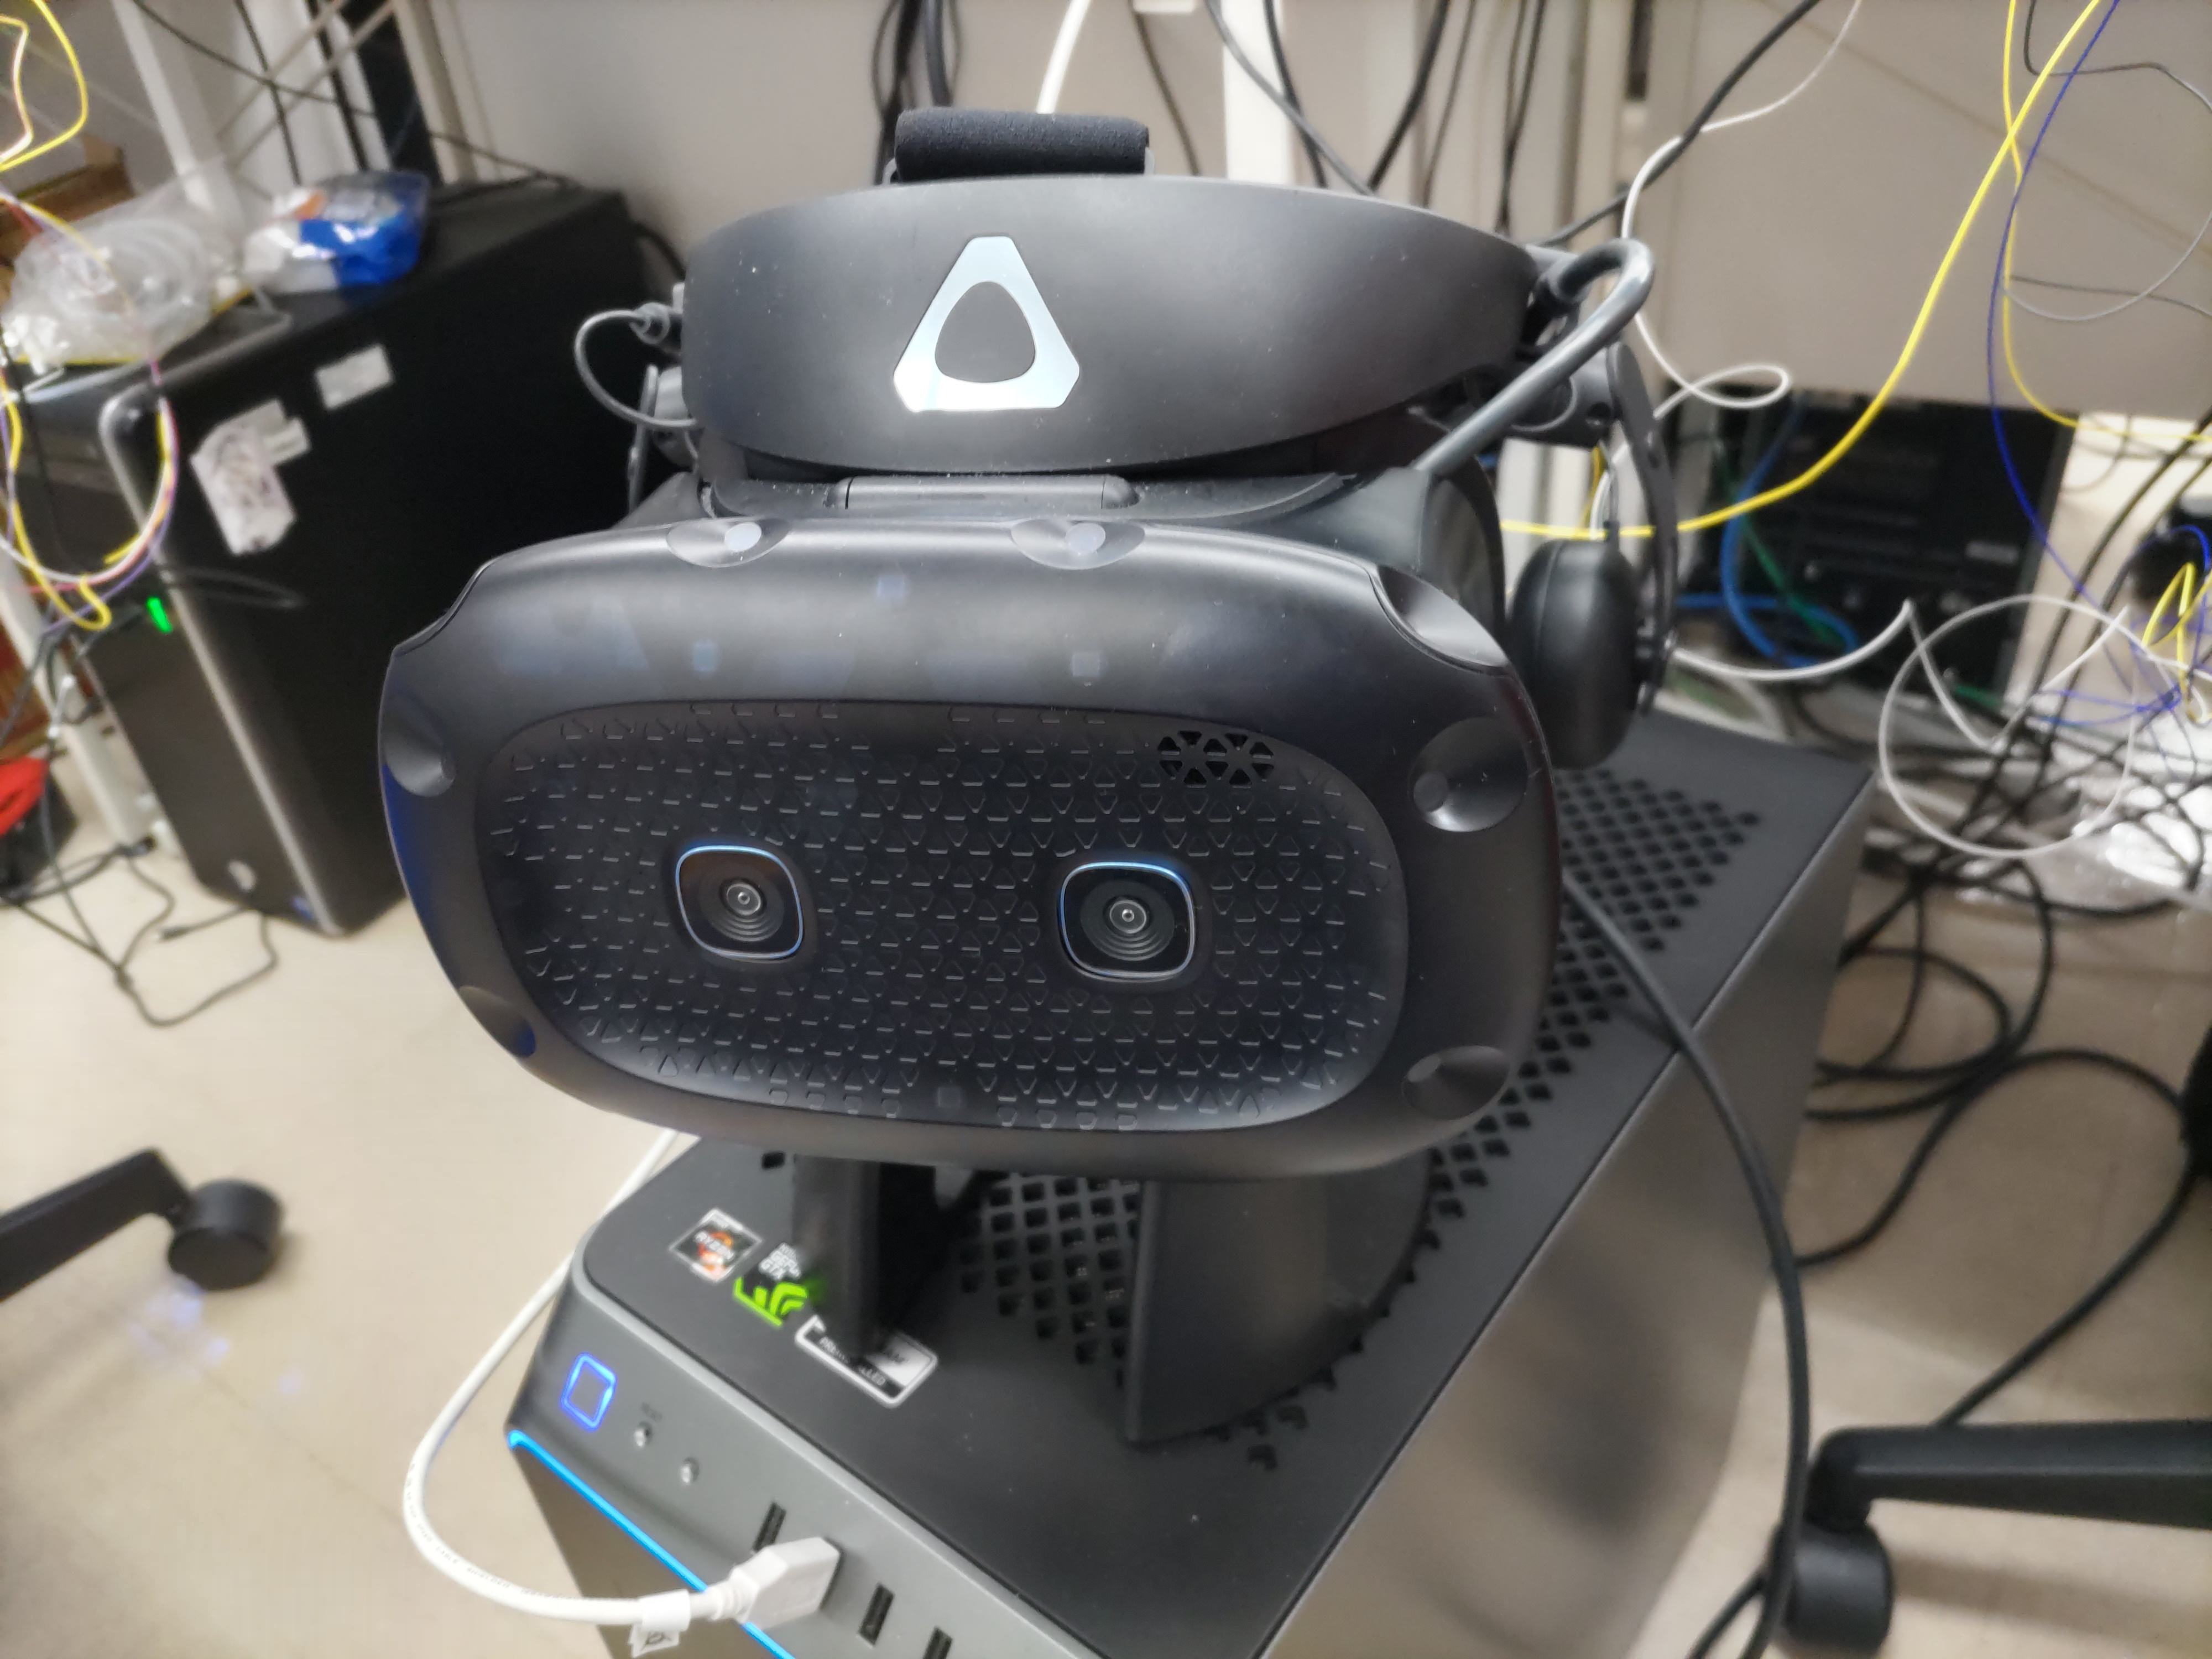
\includegraphics[clip,width=8cm]{./fig/VIVE.png}
\caption{VIVE Cosmos Elite}\label{vive}
\end{figure}

本研究で使用したヘッドマウントディスプレイ(以下HMD)をとする)を\figref{vive}に示す.
はHTC社が開発したHMDの1つである.
VR空間内での座標と方向を取得を取得し,HMDにVR空間を投影する.




\newpage

\section{振動モーター}

\begin{figure}[h]
\centering
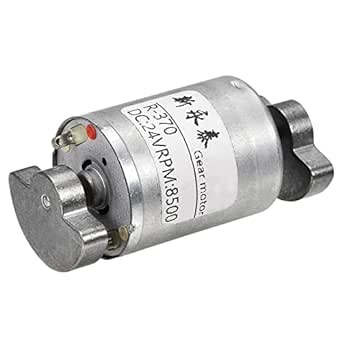
\includegraphics[clip,width=6cm]{./fig/Motor.jpg}
\caption{振動モーター}\label{motor}
\end{figure}

本研究では,ユーザーに振動刺激を与えるために振動モーターを用いる.
使用した振動モーターを\figref{motor}に示す.
振動モーターはユーザーに情報を伝えるほか,触覚フィードバックに使われる.
電流を流すと偏心重錘が回転することにより振動が発生する.


\section{Arduino}
本研究で使用したArduino UNO R3\cite{arduino}(以下Arduinoとする)を\figref{arduino}に示す.
Arduino はArduino S.L.Iによって開発・販売されているマイコンである.
USBを介してPCとの通信が可能であり,本研究ではUnityとのシリアル通信をする.

\begin{figure}[h]
\centering
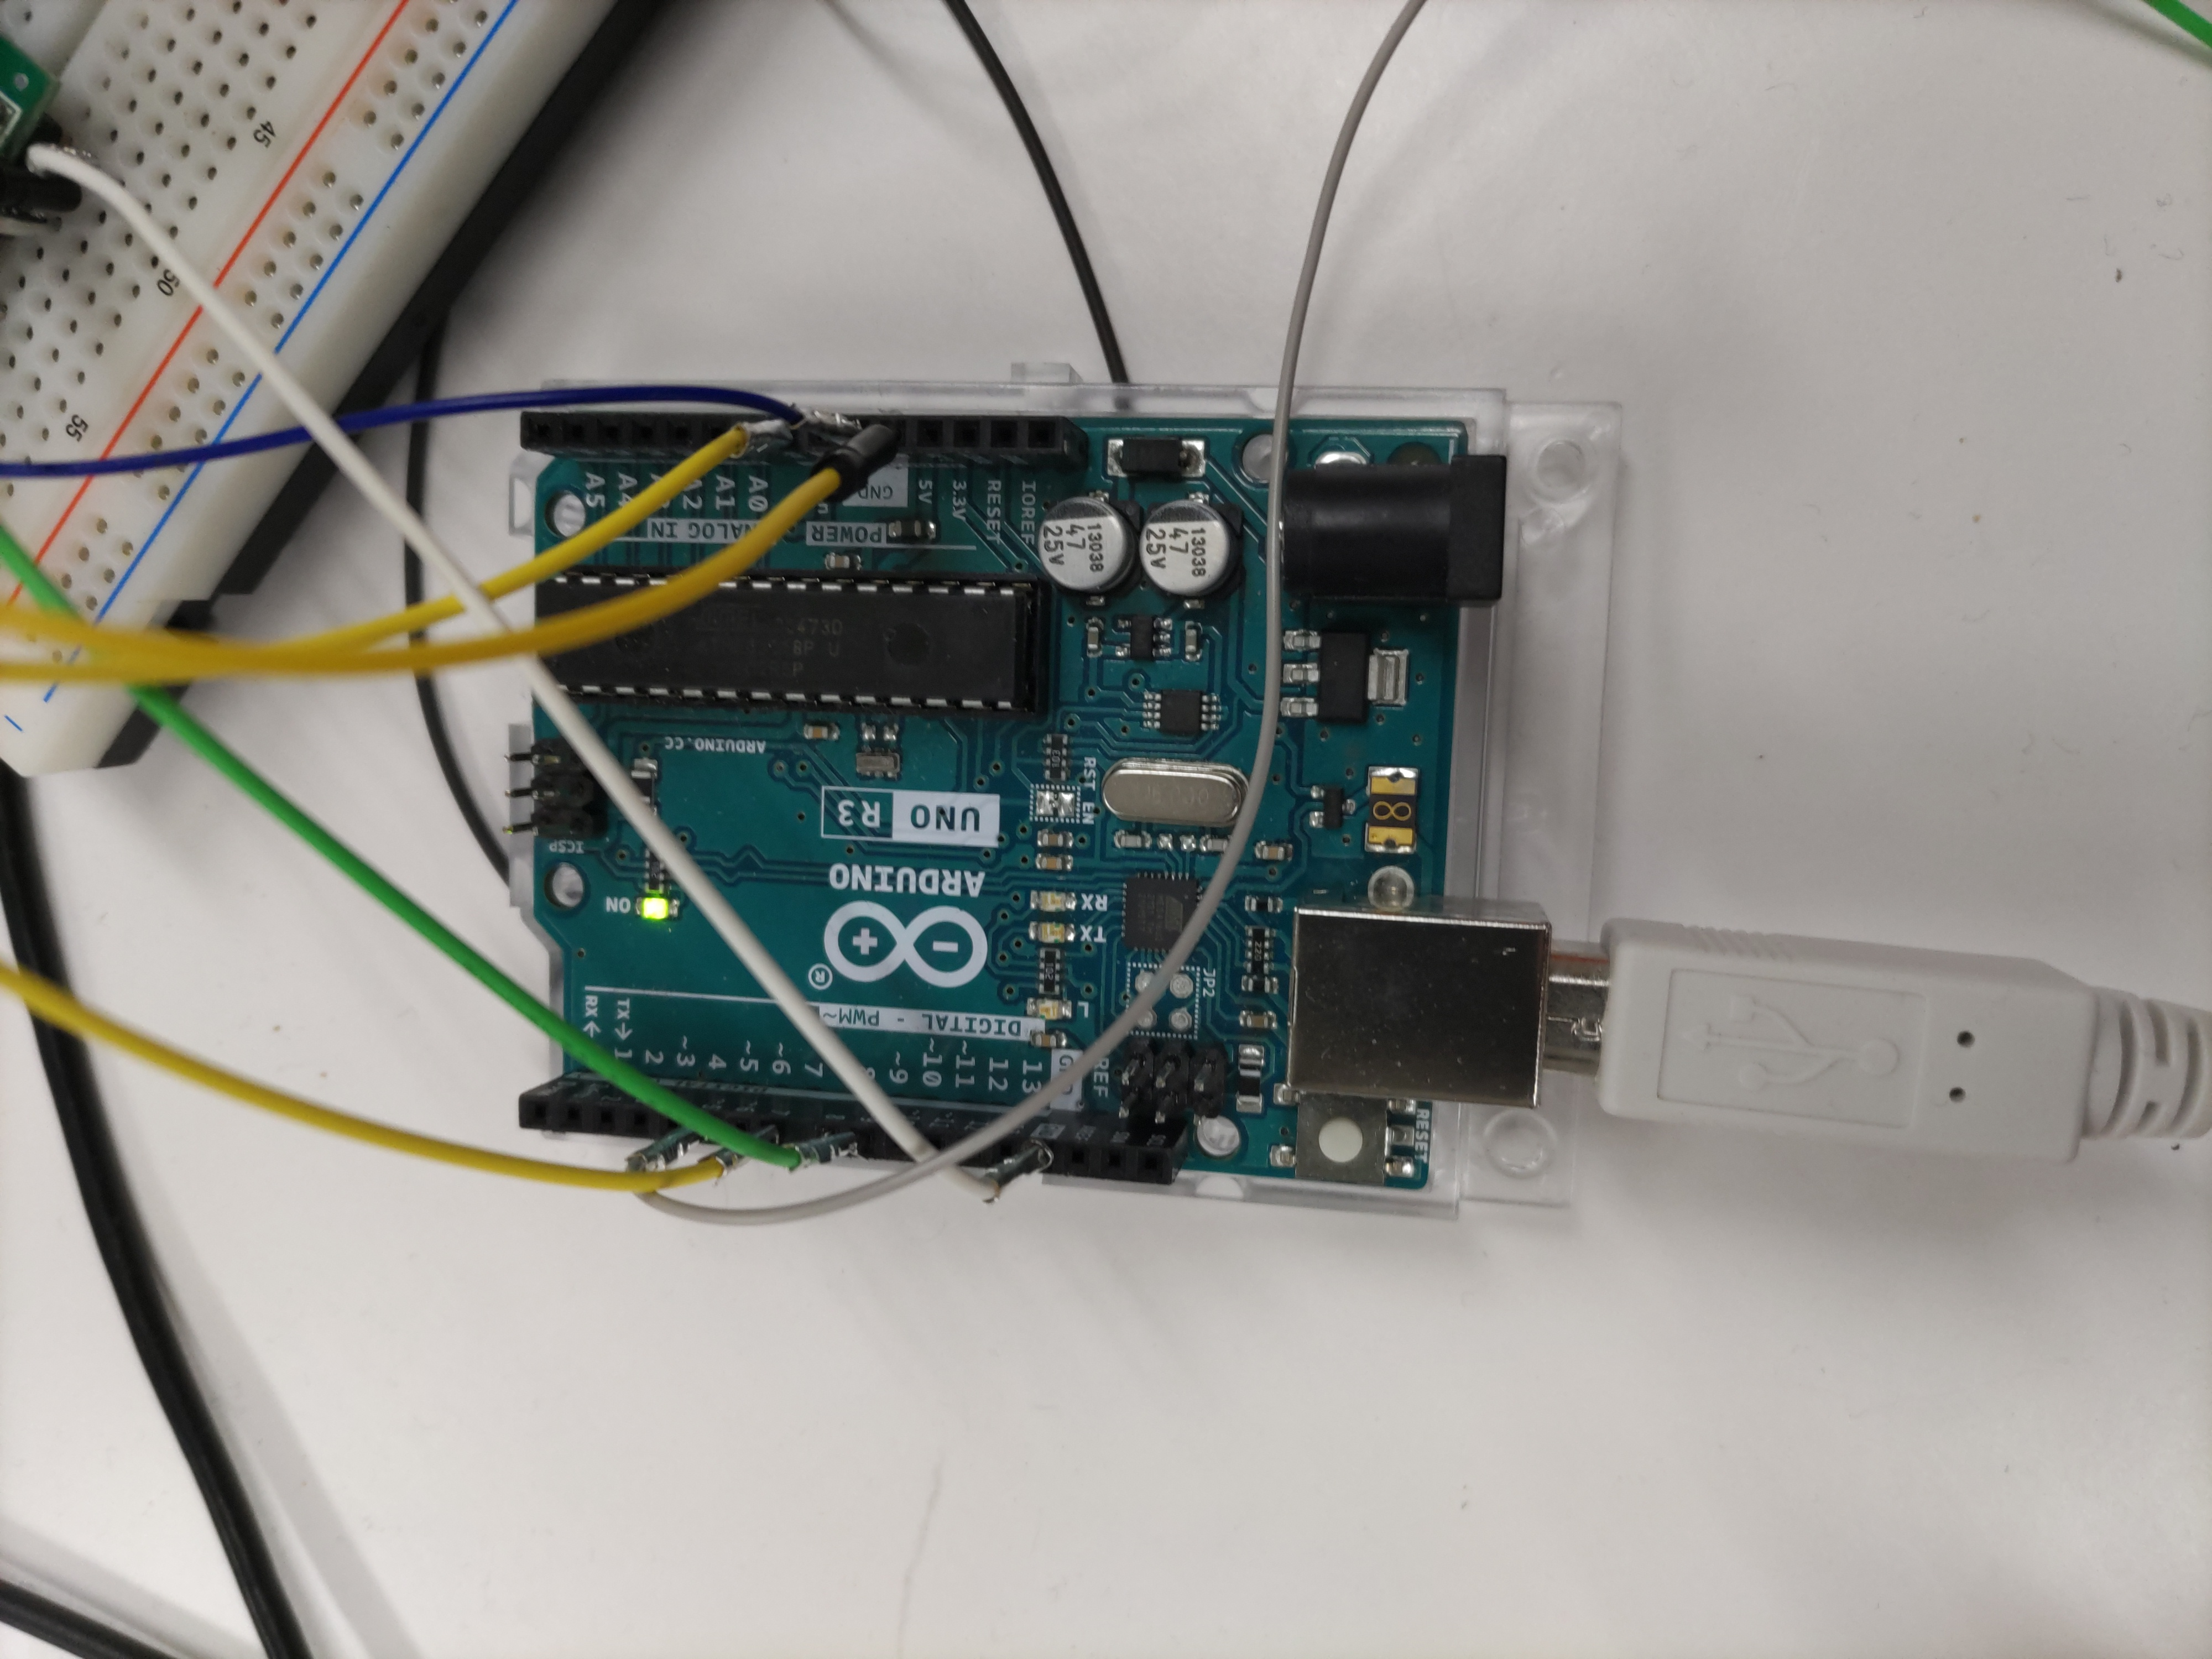
\includegraphics[clip,width=8cm]{./fig/Arduino.png}
\caption{Arduino UNO R3}\label{arduino}
\end{figure}

\newpage

\section{モータードライバ}

\begin{figure}[h]
\centering
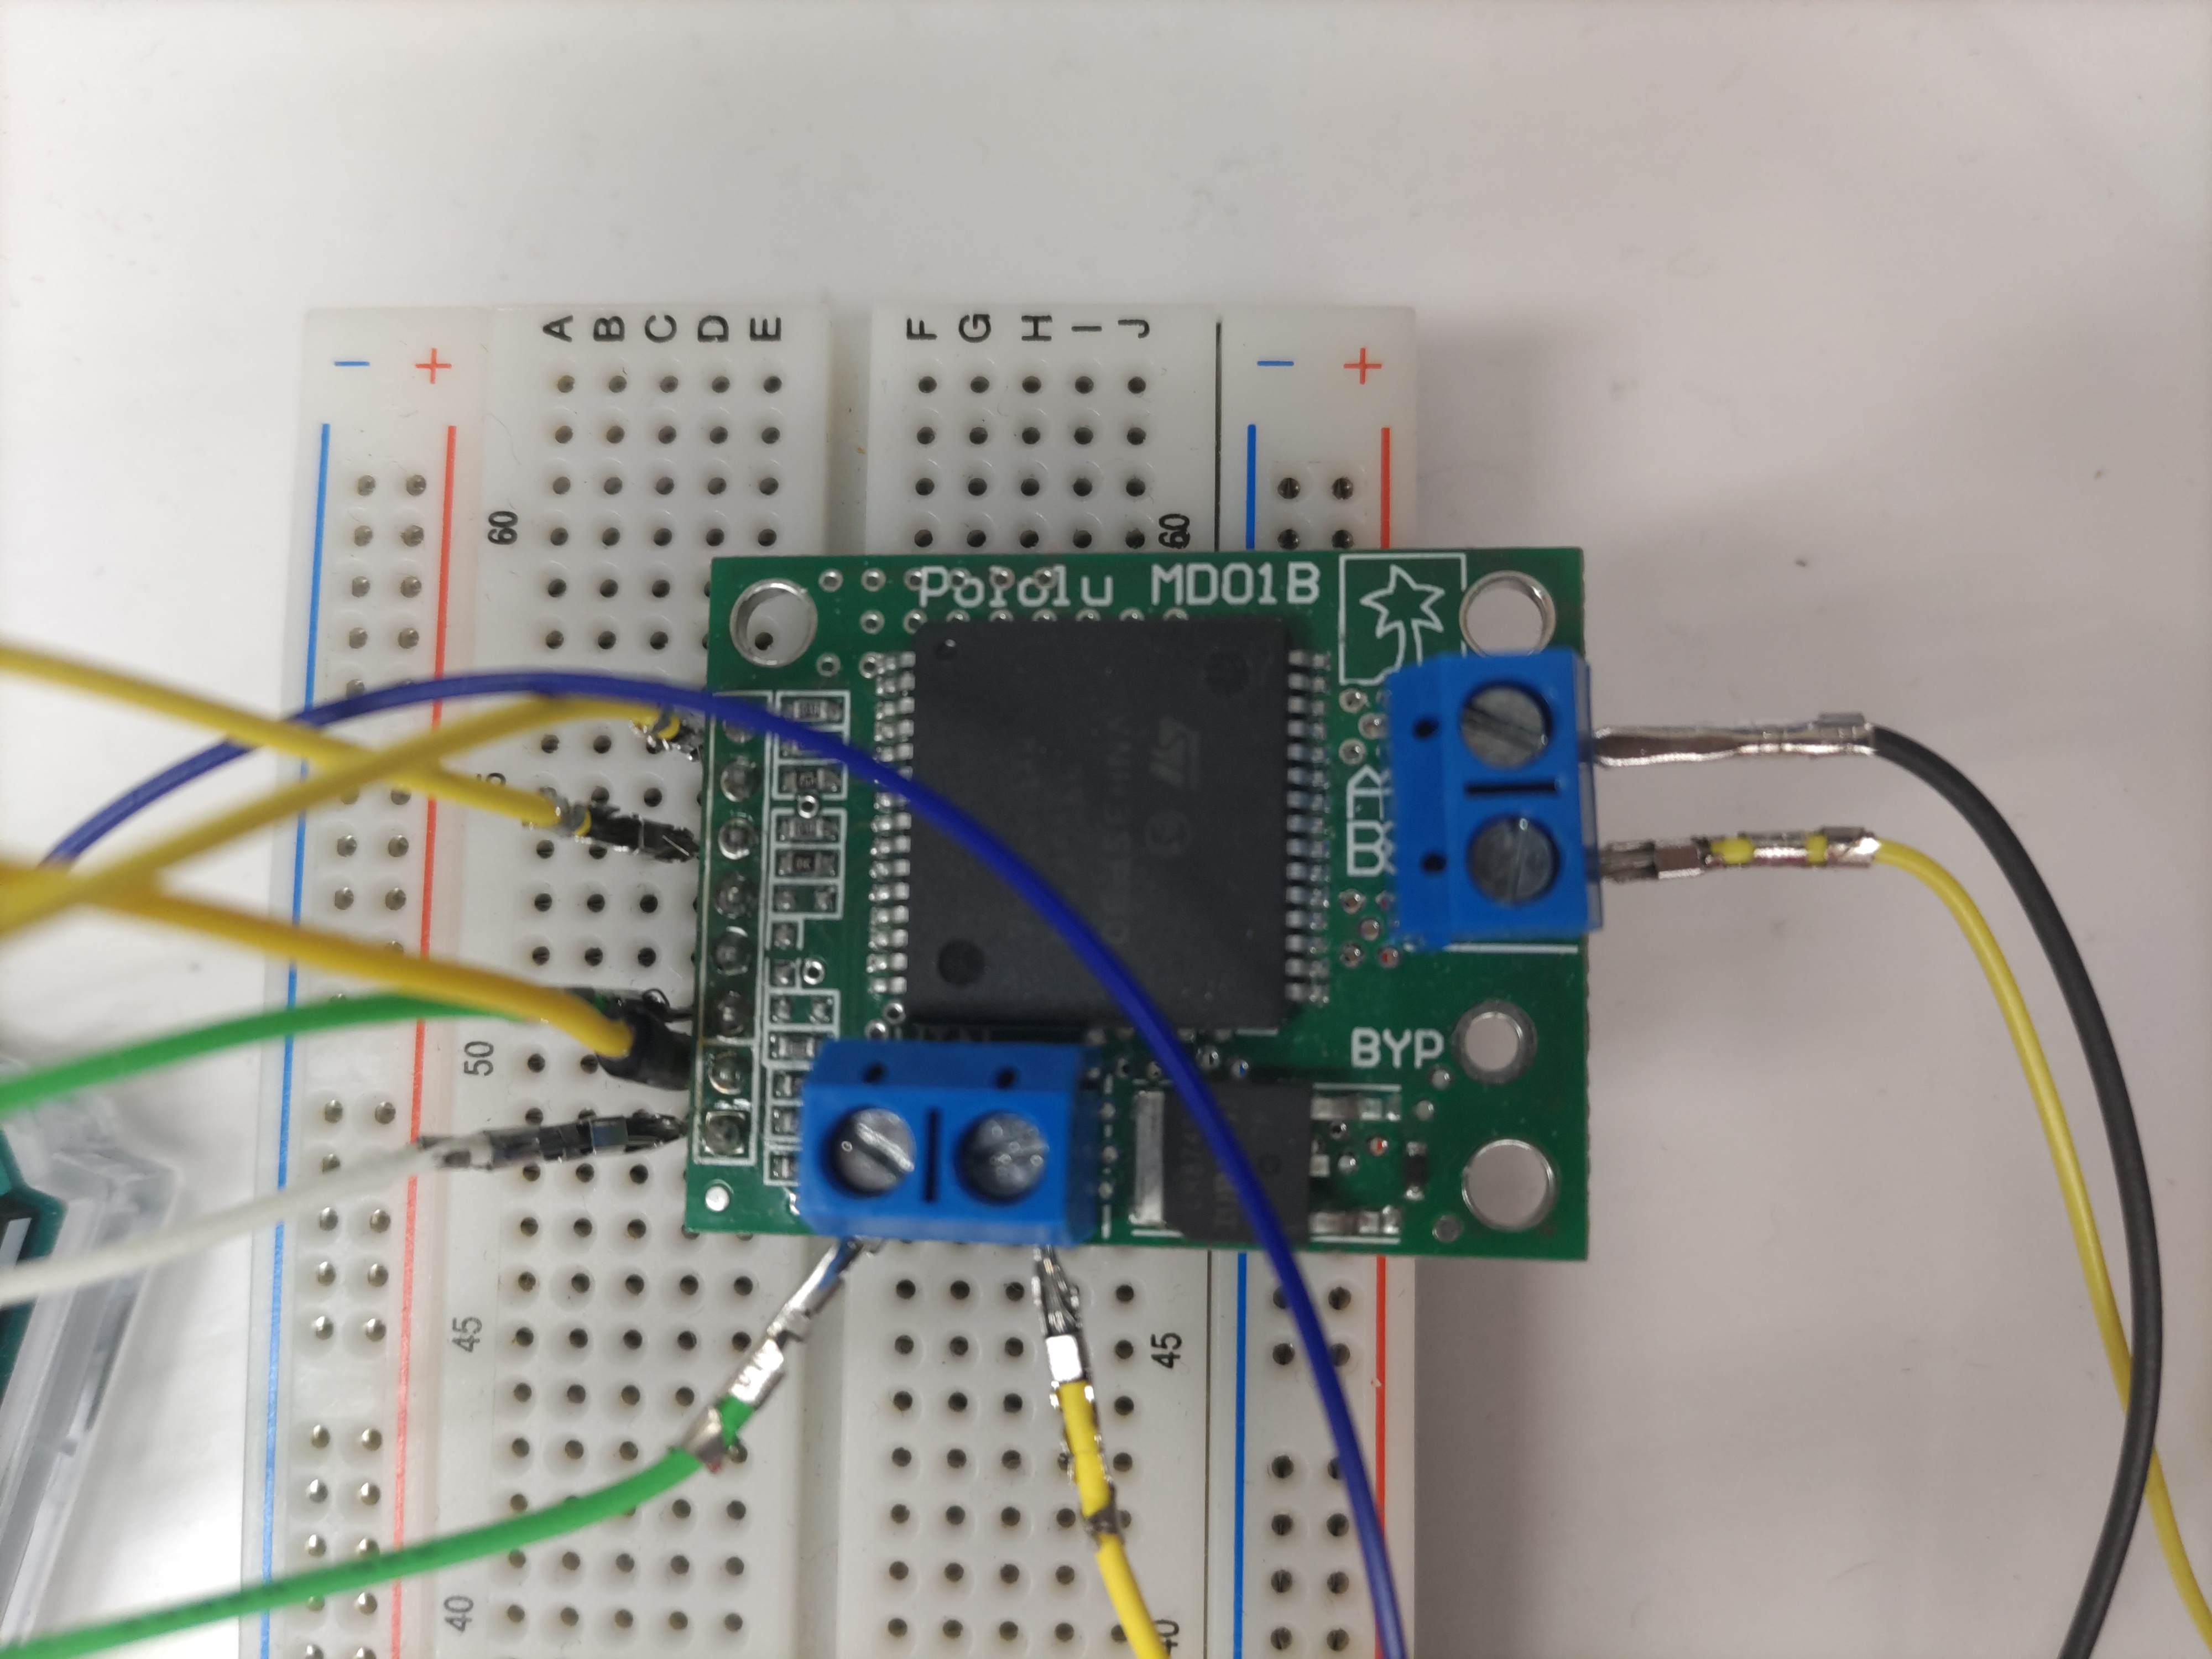
\includegraphics[clip,width=8cm]{./fig/pololuMD01B.png}
\caption{Pololu MD01B}\label{polo}
\end{figure}

\figref{polo}にモータードライバを示す.
モータードライバはArduinoからの制御信号を受け取り,電動モーターを制御する.
本システムでは,数種類の振動刺激を実装するために使用する.

\section{Unity}

\begin{figure}[h]
\centering
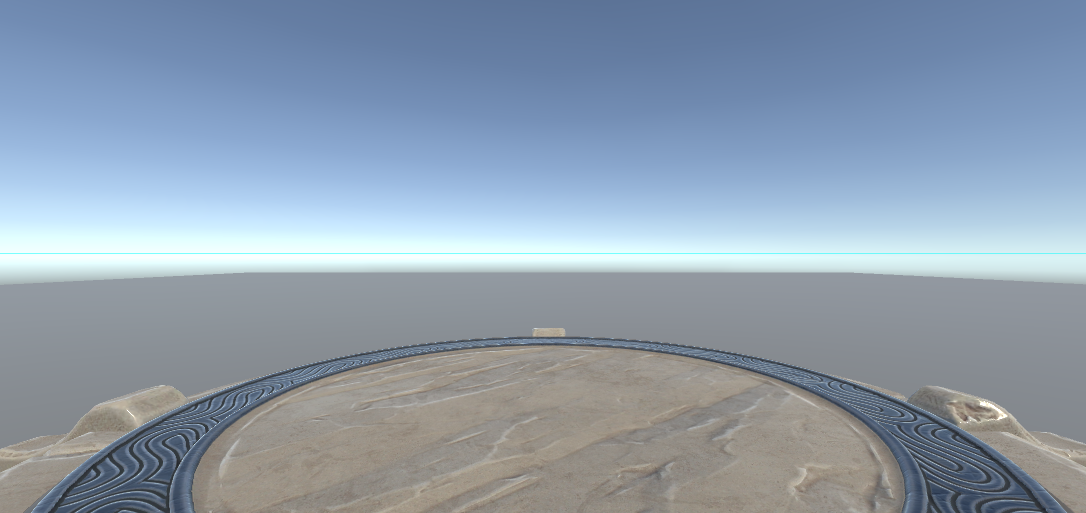
\includegraphics[clip,width=8cm]{./fig/unity_first.png}
\caption{Unity上の画面}\label{unity}
\end{figure}

Unity\cite{unity}はUnity Technologies社が開発・販売しているゲームエンジンである.
ゲーム開発や仮想現実・拡張現実などのアプリケーションを開発するためのゲームエンジンである.
プログラミングの初心者からプロの開発者まで利用しやすいため,学習や教育の分野でも利用されている.

Unityの開発画面を\figref{unity}に示す.

\section{スマートフォンにおける多様な振動フィードバックが被験者の印象に与える影響}
スマートフォンにおける多様な振動フィードバックが被験者の印象に与える影響\cite{smart}の研究を白神らが行った.
この研究では振動パターンがユーザーに与える印象について焦点を当て,約250通りの振動パターンからユーザーがどのような印象を持ったのかを調査したものである.


しかし,この研究は,スマホという掌の上での振動でしかなく,さらに大きな物体での振動についての調査は行っていない.
また,実際に存在しているものに関する振動についての調査なので,魔法という非現実的なものに対する振動については明かされていない.





